\chapter{Visualizers}

To show the capabilities or our designed \emph{framework} and \emph{platform}, we decided to implement two concrete visualizers: D3.js Chord Visualizer and Google Maps Visualizer.

\section{D3.js Chord Visualizer}

The D3.js Chord Visualizer is a brand new \emph{visualizer} that has not existed before in LinkedPipes Visualization. The core of this \emph{visualizer} is a chord diagram which is a method of visualizing the relationships among a group of entities (the data are usually represent using a square matrix). The diagram is in a form of a circle around which the entities are drown. The relationships between the entities are represent using arcs connecting them.

\begin{figure}
	\centering
	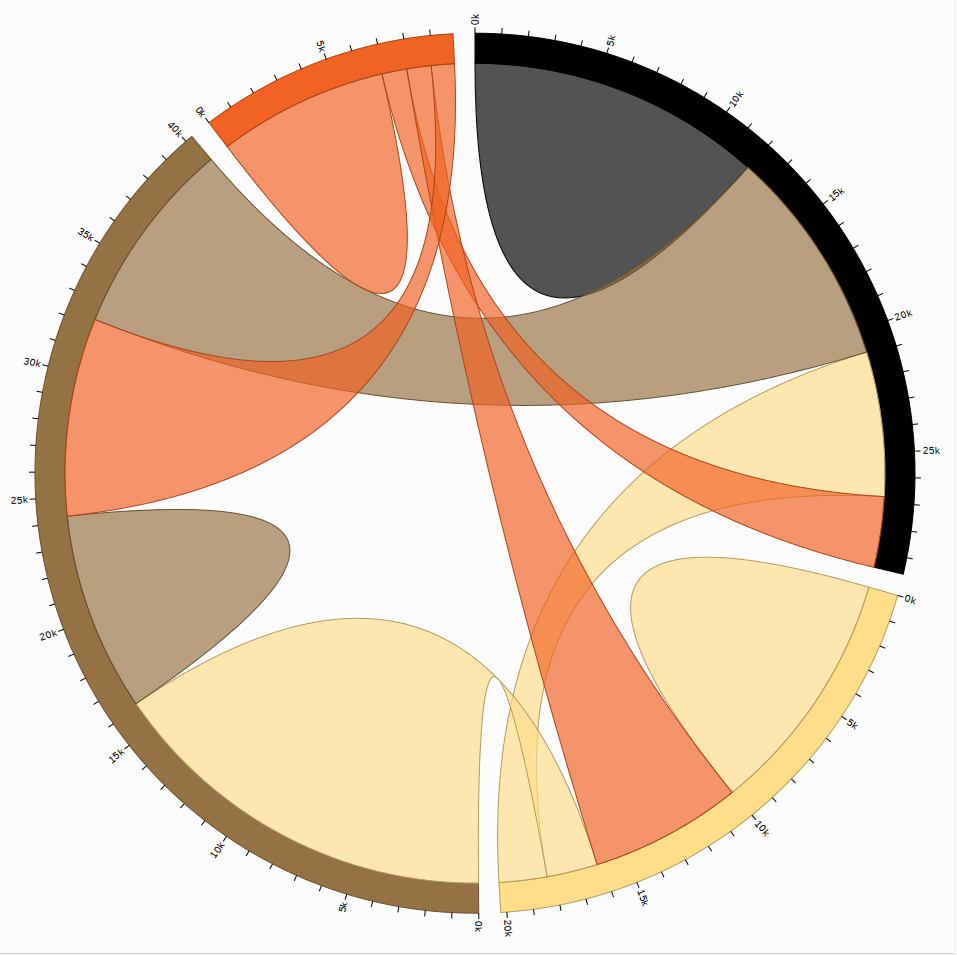
\includegraphics[width=110mm]{img/06_chord_example.png}
	\caption[Sample chord visualization]{Sample chord visualization (image source\footnotemark)  }
	\label{fig:chord-example}
\end{figure}

\footnotetext{http://bl.ocks.org/mbostock/4062006}

\subsection{Sample data sets}

We used three different data sets to demonstrate the abilities of this \emph{visualizer}.

\begin{enumerate}

\item \textbf{Registry of contracts of Czech Republic}
% [cite: http://internal.opendata.cz/dataset/gov-cz-smlouvy]

Database of contracts between private businesses and public government organizations (ministries, towns etc). The chord diagram could be used to visualize economic activity between individual business entities.

\item \textbf{UNHCR Population Statistics – Asylum seekers by months} 
% [cite: http://popstats.unhcr.org/en/asylum_seekers_monthly]

This database contains information about people from all over the world asking for asylum outside of their home countries. The database contains concrete numbers of people coming from one country to another, divided by months. The chord visualizer would be able to nicely visualize the trends of people moving around the globe.
% * <tobiaspotocek@gmail.com> 2016-06-27T15:29:26.094Z:
%
% > globe
%
% Jirka Helmich: kde jste ho vzal, jak jste ho vyrobil, citace ETL http://2016.eswc-conferences.org/sites/default/files/papers/Accepted%20Posters%20and%20Demos/ESWC2016_DEMO_Linked_Pipes_ETL.pdf
%
% ^ <tobiaspotocek@gmail.com> 2016-06-27T15:29:46.740Z:
%
% Toto zmiňuji o něco dále. Jakým způsobem jsou data sety převedeny do RDF a do RGML vocabulary. Musím to nějakým způsobem zmínit už zde?
%
% ^.

\item \textbf{OpenFlights – Air routes} 
% [cite: http://openflights.org/]

Database of airports and air routes between them from all over the world. Although air routes are not as informative as actual passenger numbers between individual destinations (that information is to our best knowledge not available), they still give a pretty good idea about overall traffic and people movements. Using a chord diagram, we can visualize traffic intensity between individual airports. This data set is also by far the largest one, consisting of around 8000 airports and almost 70000 air routes.

\end{enumerate}
These data sets are very different but they all contain information about some kind of relations which can be (with various results) visualized using a chord diagram. 

\subsection{LDVM visualizer component}

As this \emph{visualizer} was completely new, we had to start by defining the LDVM \emph{visualizer component}.

The core aspect is defining the component \emph{descriptor}, i. e., what the data should look like so that our \emph{visualizer} can visualize it. Obviously, our goal was to design a universal visualizer that could work with any data containing relationships, not just the three mentioned data sets. Therefore we focused on describing the universal shared nature of the data.

In the very beginning, we were considering the option of creating a brand new RDF vocabulary. The chord visualization was pretty uncommon in the world of Linked Data, so it would be justifiable to come up with a specialized vocabulary. Nevertheless, after some further analysis we came to realization that what the chord diagram actually visualizes is a weighted (optionally directed) multi-graph (as understood in the graph theory).

Let us look at our data sets again:

\begin{itemize}
\item The main entity in the Registry of contracts is (not surprisingly) a contract. A contract has two parties. The transition to graph vocabulary is very clear here. A contract is an edge, each party is a vertex. In this case, the graph is undirected as the partners are equal. There can be multiple contracts between two parties, so it is a multi graph. As we are not interested in the individual contracts, but rather in the number of them, all contracts between two parties could be aggregated into a single weighted undirected edge.
\item The asylum seekers data set consists of individual records where each record contains a period of time, country of origin, country of asylum and a number of people stating how many people sought asylum during that period of time between those two countries in this specified direction. Clearly, each record corresponds to an edge and each country corresponds to a vertex. The weight of an edge represents number of people. Unlike in the previous example, this time the graph is directed as it actually matters which direction the people went. Therefore a relationship between two vertices is asymmetrical. That can also be visualized using the chord diagram.
\item The air routes data set is a combination of the previous two cases. Each air route corresponds to an edge which is directed but is not by default weighted. To express the strength of a relationship, all edges of the same direction between two airports should be merged into one weighted edge.
\end{itemize}

% [cite: http://www.cs.rpi.edu/research/groups/pb/punin/public_html/RGML/EXTREME/rgml_ext.html]
Now that we had described the actual universal nature of the data visualizable by the chord diagram (a graph), it became much clearer what kind of vocabulary we would need. We were pretty certain that we would hardly be the first with the need to describe a graph in RDF. Unsurprisingly, it did not take us long to come across the RGML vocabulary which was designed with this exact purpose in mind.

\subsection{Describing graphs using RGML vocabulary}

Let us briefly describe the vocabulary. It contains these three most important classes: \texttt{rgml:Graph}, \texttt{rgml:Node} and \texttt{rgml:Edge}. The purpose of those classes is self-explanatory, nevertheless, we would like to make two remarks. Firstly, until now we have been using the term \emph{vertex} which is probably more common in graph theory. To maintain consistency with the RGML vocabulary, from now on, we will strictly stick to the term \emph{node}. Secondly, whenever we will use the term graph, we will be speaking about an actual graph structure described using the RGML vocabulary, not the RDF named graph.

The vocabulary also defines several different properties but we will describe only those most important ones. Each edge can define its source node and target node using properties \texttt{rgml:source} and \texttt{rgml:target}. Clearly, an edge is intrinsically directed. The question is whether it should be also always understood as directed. That is defined by a graph boolean property \texttt{rgml:directed}. The vocabulary allows to use this property also directly on edges which makes it possible to create mixed graphs, i. e., graphs containing both directed and undirected graphs. We did not find this feature useful for our purposes so we do not support it. There is also the \texttt{rgml:label} property which we decided to ignore and use  \texttt{rdfs:label} instead. One of the reasons was that the \emph{framework} (see Subsection \ref{sec:implementation:advanced-features:label-dereferencering}) would not be able to automatically fetch missing labels defined with the \texttt{rgml:label} property.

Let us now have a look at a concrete example. This is a data sample from the registry of contracts data set:

\begin{verbatim}
PREFIX gr: <http://purl.org/goodrelations/v1#>
PREFIX rejstriky: <http://linked.opendata.cz/ontology/domain/seznam.gov.cz/rejstriky/>
PREFIX profiles: <http://linked.opendata.cz/ontology/buyer-profiles/>
PREFIX smlouvy: <http://linked.opendata.cz/resource/domain/seznam.gov.cz/smlouvy/>
PREFIX businessentity: 
    <http://linked.opendata.cz/resource/domain/seznam.gov.cz/rejstriky/business-entity/>

<http://linked.opendata.cz/resource/business-entity/CZ00283924> a gr:BusinessEntity ;
    rejstriky:smlouva smlouvy:260167803 
    .
        
smlouvy:260167803 a rejstriky:Smlouva ;
    rejstriky:partner businessentity:67028144 
    .
\end{verbatim}

The second resource of type \texttt{rejstriky:Smlouva} is a contract between the first entity (the one of type \texttt{gr:BusinessEntity}) and the entity marked as \texttt{rejstriky:partner} of the contract. Augmented with the RGML vocabulary, the data would look like this:

\begin{verbatim}
PREFIX rgml: <http://purl.org/puninj/2001/05/rgml-schema#> .
PREFIX smlouvy: <http://linked.opendata.cz/resource/domain/seznam.gov.cz/smlouvy/>
PREFIX businessentity: 
    <http://linked.opendata.cz/resource/domain/seznam.gov.cz/rejstriky/business-entity/>

smlouvy:260167803 rdf:type rgml:Edge ;
    rgml:source <http://linked.opendata.cz/resource/business-entity/CZ00283924> ;
    rgml:target rejstriky:partner businessentity:67028144 ;
    rgml:weight "1" 
    .
    
<http://linked.opendata.cz/resource/business-entity/CZ00283924> rdf:type rgml:Node .
businessentity:67028144 rdf:type rgml:Node . 
\end{verbatim}

We used the word \emph{augmented} on purpose because we believe that it perfectly describes what happened here. We did not add any information that was not already there. We just used a different vocabulary to express the same information. A vocabulary that our visualizer understands.

Nevertheless, it is clear that some kind of data transformation has to be performed. For this particular data set we created a reusable LDVM analyzer component that is responsible for this augmentation. That means that it can take any data in the suggested format and enhance it with the RGML vocabulary to make it understandable by the chord \emph{visualizer}.

\section{Google Maps Visualizer}
% * <tobiaspotocek@gmail.com> 2016-06-27T13:27:17.697Z:
%
% > Google Maps Visualizer}
%
% Visualizer ještě projde nějakým tím lehkým faceliftingem, tak teprve pak doplním obrázky do kapitoly.
%
% ^.
Google Maps Visualizer focuses on visualizing geospatial information. It shows RDF resources containing GPS coordinates on a map in a form of markers. If the data set supports it, it allows the user to filter the resources.

This \emph{visualizer} was already implemented in LinkedPipes Visualization, so we were able to re-use the LDVM \emph{visualizer component} definition and also all the backend code responsible for extracting RDF data from the \emph{pipeline evaluation}. We only had to implement the frontend part, specifically the \emph{configurator} and \emph{application} interfaces.

For these reasons, this chapter will be rather short and it will not go into technical details. Instead, we will rather focus on the comparison between the original \emph{visualizer}, which is part of LinkedPipes Visualization, and our own implementation that utilizes the capabilities of the \emph{application generator}. 

\subsection{Sample data set}

We will demonstrate the capabilities of this \emph{visualizer} using only a single data set, \textbf{Registry of business subjects in Czech Republic} [cite and use the real name]. As the name suggests, this data set contains business subjects. Each business subject has GPS coordinates of its residence. These entities will be visualized on the map.

Each business subject is put into two categories. The \emph{primary category} and the \emph{secondary category}. The data set contains list of available categories. The user will be allowed to filter the business subjects using these categories.

\subsection{Filtering}

Filtering is an essential part of this \emph{visualizer}. It works similarly to what the reader might be used to for example from browsing products in e-shops. Just for now, let us say that the data set does not contain geospatial entities but rather laptops. A laptop has properties like brand, screen size or operating system. Each of these properties defines a \emph{filter} (e.g. brand) with a list of available \emph{values} (e.g. Asus, Dell, Apple etc). The user can select an arbitrary number of \emph{values} for each \emph{filter} to create filtering criteria. For a laptop to be included in the result set, it has to match all the criteria (conjunction). For a laptop to match a criterion, its property \emph{value} corresponding to the criterion \emph{filter} must be one of the \emph{values} selected by the user (disjunction). For example, by selecting Asus and Dell as the brand, 15 inches as the screen size and Windows 10 as the operating system, the user will get all 15-inch laptops with Windows 10 manufactured either by Asus or Dell.

If the user selects all \emph{values} for a \emph{filter}, it is just as if the \emph{filter} was not there at all. It has no impact on the result set. On the other hand, if the user selects no \emph{values} for a \emph{filter}, the results set is always empty (no laptops can meet the criteria).

Available \emph{filters} and their \emph{values} has to be explicitly defined in the data set. In our sample data set, as already mentioned, those are the \emph{primary category} and \emph{secondary category}.

\subsection{Configurator and application user interface}

\emph{Configurator} and \emph{application} interfaces are very similar. Both of them feature a map and a sidebar on the left with \emph{filters}. The key difference is that in the \emph{configurator} interface, the \emph{filters} can be displayed in two modes: configuration and preview. The \emph{application} interface shows the \emph{filters} always in the same way which corresponds to the preview mode.

The idea is that by configuring the \emph{filters} the user can significantly affect the shape of the published application. Here are some examples.

\begin{itemize}
\item A \emph{filter} can be \textbf{disabled}. A disabled \emph{filter} is interpreted as if all its \emph{values} have been selected, i.e., it has no impact on the selected output. This filter is completely hidden in the published application.
\item A \emph{value} can be \textbf{enforce}. That means that it is always selected.
\item A \emph{value} can be \textbf{disabled}. That means that it cannot be selected. This \emph{value} is completely hidden in the published application.
\item A \emph{filter} can be switched between \textbf{checkbox} mode and \textbf{radio} mode. In checkbox mode, an arbitrary number of \emph{filter} \emph{values} can be selected. In radio mode, only one \emph{value} can be selected. The mode names correspond to the appropriate form controls.

\end{itemize}
Thanks to the enforcing and disabling of certain \emph{values}, it is possible to create default filters that are always applied. That essentially means that the published application can be based just on a subset of the input data. If we go back to our example with laptops, one could generate a browser of Dell laptops filterable by screen size. To achieve that, one would have to disable the operating system \emph{filter}, enforce the Dell \emph{value} and disable all other \emph{values} for the brand \emph{filter}.

By either fixing or disabling all \emph{filters} and \emph{values}, it is actually possible to generate a completely static application which might also make sense in certain situations. Moreover, It is possible to disable the sidebar with \emph{filters} completely which reduces the published application just to a static map with pre-selected markers.

Besides the filter configuration, the \emph{configurator} interface also allows the user to fix the default map position and zoom level. Naturally, it also implements the available universal features, like multi language support and custom labels editor (e.g. it is possible to rename \emph{filters}  and their \emph{values}).

% TODO: marker infowindows/tooltips

\subsection{Advantages over LinkedPipes Visualization}

The reader might be wondering why we presented a sample data set but then we used a completely different example to explain how the filtering works. The reason is that the presented data set is if not actually broken then at least very confusing (its quality is a little poor). That does not make it very suitable for explaining principles, but it makes it perfect for demonstrating the abilities of our \emph{visualizer}.

As explained, each business subject has a \emph{primary category} and a \emph{secondary category}. Those are two properties that would both make up one \emph{filter} each. Since the data is in RDF, each property is actually an RDF resource with a unique URI. The problem here is that they both have the same label and they both contain exactly the same \emph{values} which means that they will both look exactly the same to the user. The label can be approximately translated as \textit{"Businesses as defined by the 1st attachment of the integrated prevention law"}.

If we go back to the example of the e-shop selling laptops, there is one big assumption: We assume that the user is at least to some extent familiar with the nature of the product. E.g. he knows what the brand or the screen size is. Therefore we assume that he would intuitively understand what happens if he selects in the filters the brand Dell and the screen size 15 inches. In case of our data set, however, not only might the user have no idea what \textit{"Businesses as defined by the 1st attachment of the integrated prevention law"} are in the first place, but also the fact that this property is there twice would confuse him even more. 

It is important to say that this is exactly what the LinkedPipes Visualization visualizer would show. Two identical \emph{filters} with confusing names and identical \emph{values}. We can hardly expect any intuition from the user here. Plus the list of \emph{values} is fairly long and because of the way it is displayed, the user might not realize that there are actually two \emph{filters}. That might cause another problem: if the user is not aware of the second \emph{filter} and selects no \emph{values} for it, he will always get an empty result set.

Interestingly enough, the current implementation in LinkedPipes Visualization does not suffer from this problem but only by a sheer coincidence. Firstly, even though each business subject is put into two categories (\emph{primary} and \emph{secondary}), they are always the two same categories, i.e., both the \emph{primary} and the \emph{secondary category} points to the same RDF resource with the same URI. Secondly, there is a bug in the  user interface implementation of filters in LinkedPipes Visualization causing that if the user selects a \emph{value} in the \emph{primary category} \emph{filter}, this \emph{value} (identified by a URI) gets also automatically selected in the \emph{secondary category} \emph{filter}.

In the example with laptops this would mean that each laptops would have two brands which would however be always the same (e.g. a laptop would have the "primary" brand Dell and also the "secondary" brand Dell). To filter Dell laptops, we would need to specifically select Dell in both brand \emph{filters}. Because of the UI bug, this would be done automatically for us.

The reader might object that this behavior in the UI is not a bug but is rather intentional as it follows the structure of the data. Let us imagine that a laptop has two new properties. A chassis color and a keyboard color. They would correspond to two new \emph{filters} with exactly the same \emph{values} (a list of several predefined colors). Clearly, we want to select the colors independently. Selecting red for the chassis should not automatically mean selecting red for the keyboard. Note that structure of this example is identical to our data set. The only difference is that our \emph{primary category} and \emph{secondary category} both have the same label, so they appear as identical. But they are not. Their URIs are different and that is what matters.

To sum it up: a visualization of this data set generated with LinkedPipes Visualization would expose all these flaws to any end user that would come across this visualization. This makes the visualization not very user friendly. On the other hand, in our \emph{application generator} we can utilize the configuration phase to fix these issues and deliver much better user experience (not to mention that our implementation does not suffer from the aforementioned bug). Specifically, we could undergo the following steps:

\begin{itemize}
\item \textbf{Rename the \emph{filters}.} Using the custom labels editor we could provide better and more explanatory names to the \emph{filters} so that the user would get a better idea of their behavior. Just using "Primary category" and "Secondary category" as names would probably improve the overall experience. The original name, \textit{"Businesses as defined by the 1st attachment of the integrated prevention law"}, rather just explains what the \emph{values} are and this information could go to the application description.
\item \textbf{Disable one of the \emph{filters}.} As in this data set both categories are always the same, disabling one of the filters will not cause the visualization to lose any information or functionality and it will only improve the experience.
\item \textbf{Reduce the data set}. Even if one of the \emph{filters} is disabled, there is still more than 60 \emph{values} to choose from. Perhaps we could instead of one big application generate multiple smaller applications where each would utilize default filters to visualize only a specific subset of the data set.
\end{itemize}

Using our \emph{application generator}, we were able to take a data set of poor quality and turn it into a useful and user-friendly application. Which is something that would not be possible with LinkedPipes Visualization.

One last remark. The \emph{configurator interface} does not shield the user from these data set related problems. The main advantage is that only the user that generates the application needs to deal with these issues. Once the application is properly generated, it is ready to be comfortably consumed by a way broader audience. In LinkedPipes Visualization, on the other hand, everybody gets the raw visualization and has to make his own sense out of the data.
